\documentclass{beamer}

\usepackage[utf8]{inputenc}
%\usepackage[latin1]{inputenc}
\usepackage{amsmath,amssymb}
\usepackage[brazil]{varioref}
\usepackage[english,brazil]{babel}
\usepackage{graphicx}
\usepackage{listings}
\usepackage{url}
\usepackage{colortbl}
\usepackage{setspace}
\usepackage{multimedia}

\mode<presentation>{
\usetheme{Dresden}
\setbeamercovered{transparent}
\usecolortheme{lsc}
}

\mode<handout>{
  \usepackage[bar]{beamerthemetree}
  \beamertemplatesolidbackgroundcolor{black!5}
}

\beamertemplatetransparentcovereddynamic
\newcommand{\frameofframes}{/}
\newcommand{\setframeofframes}[1]{\renewcommand{\frameofframes}{#1}}
\setframeofframes{de}
\makeatletter
\setbeamertemplate{footline}
  {%
    \begin{beamercolorbox}[colsep=1.5pt]{upper separation line foot}
    \end{beamercolorbox}
    \begin{beamercolorbox}[ht=2.5ex,dp=1.125ex,%
      leftskip=.3cm,rightskip=.3cm plus1fil]{author in head/foot}%
      \leavevmode{\usebeamerfont{author in head/foot}\insertshortauthor}%
      \hfill%
      {\usebeamerfont{institute in head/foot}\usebeamercolor[fg]{institute in head/foot}\insertshortinstitute}%
    \end{beamercolorbox}%
    \begin{beamercolorbox}[ht=2.5ex,dp=1.125ex,%
      leftskip=.3cm,rightskip=.3cm plus1fil]{title in head/foot}%
      {\usebeamerfont{title in head/foot}\insertshorttitle}%
      \hfill%
      {\usebeamerfont{frame number}\usebeamercolor[fg]{frame number}\insertframenumber~\frameofframes~\inserttotalframenumber}
    \end{beamercolorbox}%
    \begin{beamercolorbox}[colsep=1.5pt]{lower separation line foot}
    \end{beamercolorbox}
  }
\makeatother
\title[Sistema de coordenadas para posicionamento de instrumentos de medição em um túnel de vento]
{\normalsize Sistema de coordenadas para posicionamento de instrumentos de medição em um túnel de vento}
\author[Baldez Jr, Torma]{Alexandre Marques Baldez Junior - abaldezjr@gmail.com \and Rodrigo de Souza Torma - rstorma@hotmail.com}
\institute[FURG]{
Orientador: Prof. Dr. Gustavo da Cunha Dias\\
Co-Orientador: Prof. Me. Letieri Rodrigues de Ávila  
\and
Universidade Federal do Rio Grande\\
Engenharia Mecânica empresarial
}

\date{29 de maio de 2021}
\pgfdeclareimage[height=0.4cm]{inf}{figuras/logofurg.jpg}
\logo{\pgfuseimage{inf}}

\AtBeginSection[]{
  \begin{frame}<beamer>
    \frametitle{Roteiro}
    \tiny{\tableofcontents[currentsection, hideothersubsections, sectionstyle=show/show]}
  \end{frame}
}

\begin{document}

\begin{frame}[plain, noframenumbering]
\titlepage
\end{frame}

\begin{frame}
\frametitle{Roteiro}
\tableofcontents[currentsection, hideothersubsections, sectionstyle=show/show]
\end{frame}

\section{Introdução}

\subsection{Apresentação do tema}

%SLIDE DE APRESENTAÇÃO DO TEMA
\begin{frame}
\frametitle{Apresentação do tema}
\begin{itemize}
    \item A mecânica dos fluidos é uma área muito complexa da engenharia.
    \item Nem sempre é possível  projetar com precisão sem uma análise prévia da ação de esforços sobre algum material. 
    \item O estudo da ação do ar sobre estruturas pode ser um fator determinante para o sucesso de um projeto. 
\end{itemize}
\end{frame}

%SLIDE DE APRESENTAÇÃO DO TEMA
\begin{frame}
\frametitle{Apresentação do tema}
\begin{itemize}
    \item A análise aerodinâmica pode apresentar dados confiáveis ao projetista para tomada de decisão. 
    \item Através das leis de similaridade, aplica-se fatores de escala para replicar os resultados em escalas reais. 
    \item De uma forma menos onerosa é possível se fazer esse estudo em escala reduzida e com condições controladas em laboratório.
\end{itemize}
\end{frame}

%SLIDE DE TÚNEL DE VENTO
\begin{frame}
\frametitle{Túnel de vento}

Os túneis de vento são as bancadas de testes para estudos de escoamento de ar, onde é possível simular cenários e avaliar a interação do fluido e estrutura.

\begin{figure}
\centering
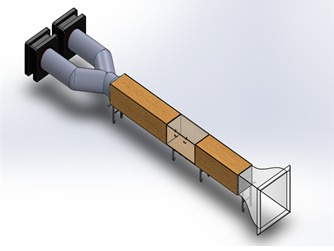
\includegraphics[scale = 0.4]{figuras/tuneldeventosombreado}
\end{figure}

\end{frame}
 
% SLIDE DOS INSTRUMENTOS DE MEDIÇÃO
\begin{frame}
\frametitle{Instrumentos de medição}

Uma das grandezas obtidas é a velocidade do fluido, a qual é medida por instrumentos como tubo de Pitot ou sonda de anemômetro de fio quente.

    \begin{columns}
        \column{0.5\textwidth}
            \begin{figure}
            \centering
            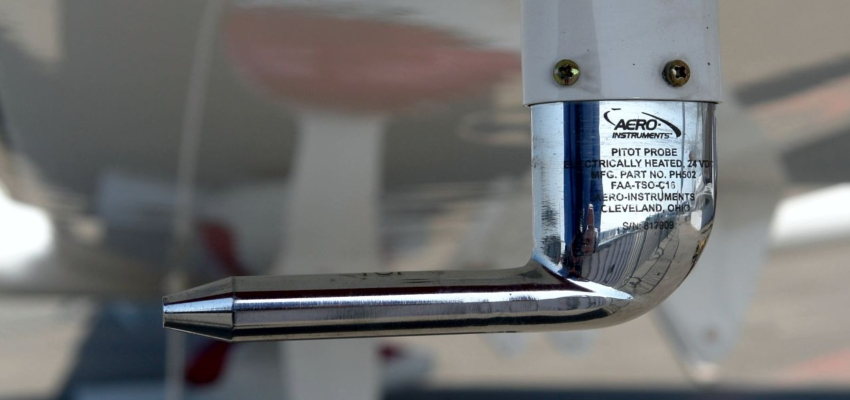
\includegraphics[scale = 0.6]{figuras/tubodepitotaviao}
            \end{figure}
        \column{0.5\textwidth}
            \begin{figure}
            \centering
            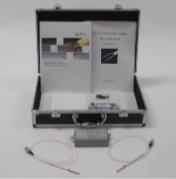
\includegraphics[scale = 0.6]{figuras/sonda}
            \end{figure}
    \end{columns}
\end{frame}

\subsection{Apresentação do problema}

%SLIDE DE APRESENTAÇÃO DO PROBLEMA
\begin{frame}
\frametitle{Apresentação do problema}
\begin{itemize}
    \item O posicionamento dos instrumentos dentro do túnel de vento é realizado de forma manual, exigindo que o operador desligue o túnel.
    \item Isso causa uma baixa repetibilidade e menor precisão. 
    \item Para tanto, propomos o desenvolvimento de um mecanismo que faça esse deslocamento dos instrumentos de medição de forma automatizada.
\end{itemize}
\end{frame}

\begin{frame}
    \frametitle{Apresentação do problema}
        \begin{figure}
        \centering
        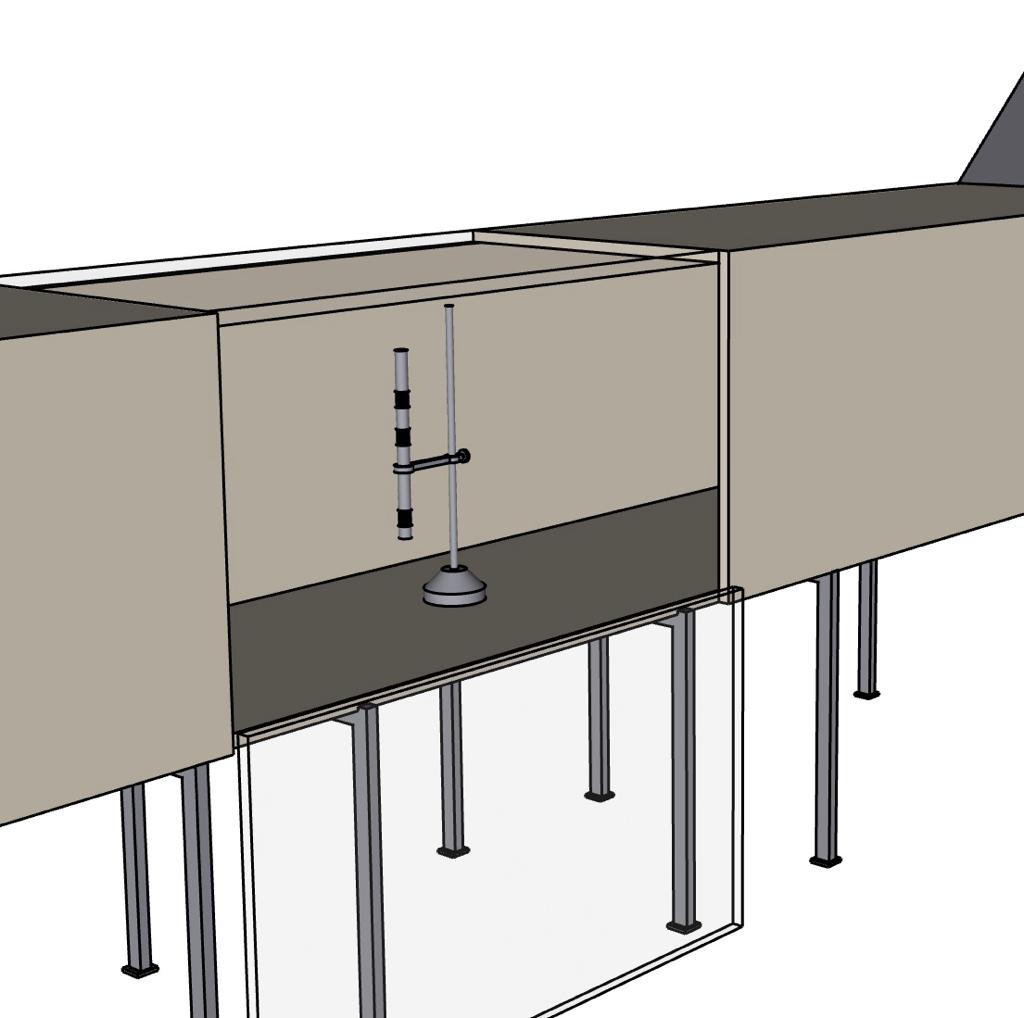
\includegraphics[scale = 0.15]{figuras/sisantigozoom}
        \end{figure}
\end{frame}
    
\subsection{Justificativa}

%SLIDE DE JUSTIFICATIVA
\begin{frame}
\frametitle{Justificativa}

A realização desse trabalho justifica-se por desenvolver um equipamento que agregue um sistema de coordenadas bidimensional para posicionamento de instrumentos de medição no túnel de vento do Laboratório de Sistemas Térmicos  da Universidade Federal do Rio Grande.

\end{frame}

\subsection{Objetivos}

% SLIDE DE OBJETIVOS
\begin{frame}
\frametitle{Objetivo geral}

Projetar um dispositivo para o posicionamento de equipamentos de medições dentro de um túnel de vento para facilitar o processo de avaliação de velocidades e pressões de forma automatizada.

Objetivos específicos:
\begin{itemize}
    \item Projetar a mesa cartesiana.
    \item Criar o sistema eletrônico de comunicação entre a mesa e o software.
    \item Desenvolver o software que comandará a mesa cartesiana.
\end{itemize}

\end{frame}


\section{Referencial teórico}

\subsection{Túnel de vento}

%SLIDE DE TUNEL DE VENTO
%\begin{frame}
%\frametitle{Túnel de vento}
%
%Os túneis de vento são estruturas que propiciam a simulação para o desenvolvimento de estudos que relacionam o efeito do movimento de ar em torno de objetos, como turbinas, aviões, carros e edificações. 
%
%\begin{itemize}
%    \item Circuito: Aberto e fechado.
%    \item Vel. escoamento: Subsônico, supersônico e hipersônico.
%    \item Para aberto: Soprador e sugador.
%\end{itemize}
%
%\end{frame}

%SLIDE DE TUNEL DE VENTO
\begin{frame}
\frametitle{Túnel de vento}

O túnel de vento tratado neste trabalho está situado junto ao Laboratório de Sistemas Térmicos da Universidade Federal do Rio Grande e é de característica subsônica, circuito aberto e do tipo soprador.

\begin{figure}
\centering
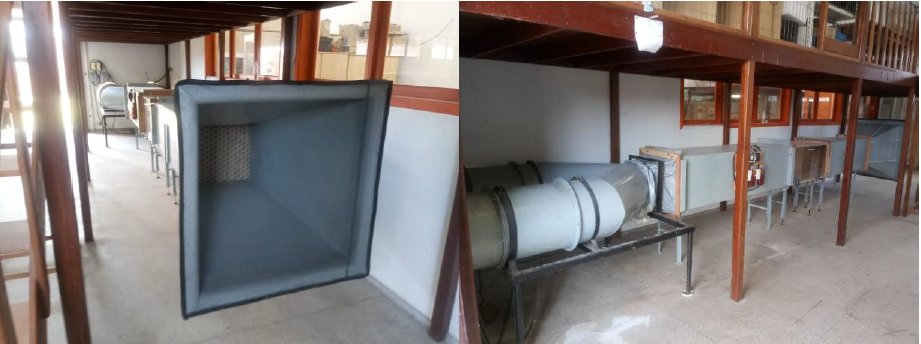
\includegraphics[scale = 0.4]{figuras/tunelfran}
\end{figure}

\end{frame}

\subsection{Tubo de Pitot}

% SLIDE DE TUBO DE PITOT
\begin{frame}
\frametitle{Tubo de pitot}

A subtração da pressão total da estática resulta na pressão dinâmica do escoamento

Pressão dinâmica = Pressão total - Pressão estática

\begin{figure}
\centering
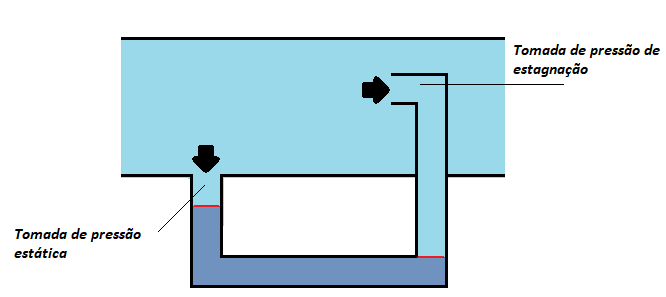
\includegraphics[scale = 0.5]{figs/pestagnacao}
\end{figure}

\end{frame}
\subsection{Mesa de posicionamento}

% SLIDE DE MESA DE POSICIONAMENTO
\begin{frame}
\frametitle{Mesa de posicionamento}

Podem ser classificadas em dois tipos com relação a sua transmissão: as mesas acionadas por fusos e por correias sincronizadas.

\begin{columns}
    \column{0.5\textwidth}
        \begin{figure}
        \centering
        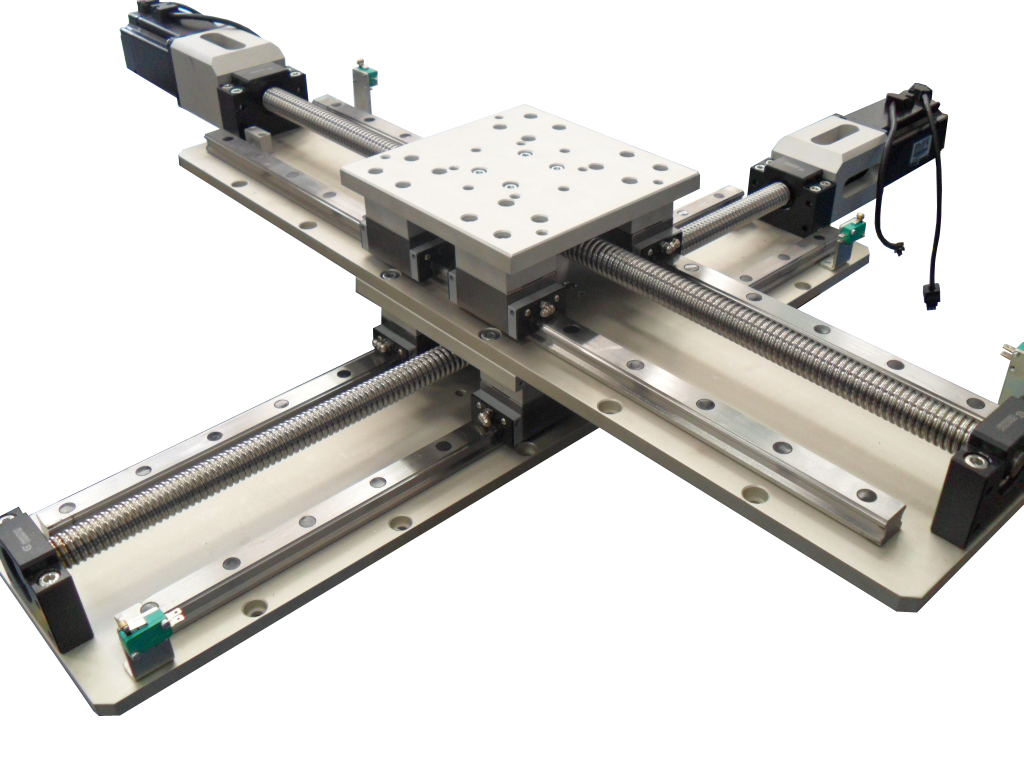
\includegraphics[scale = 0.12]{figuras/mfuso}
        \end{figure}
    \column{0.5\textwidth}
        \begin{figure}
        \centering
        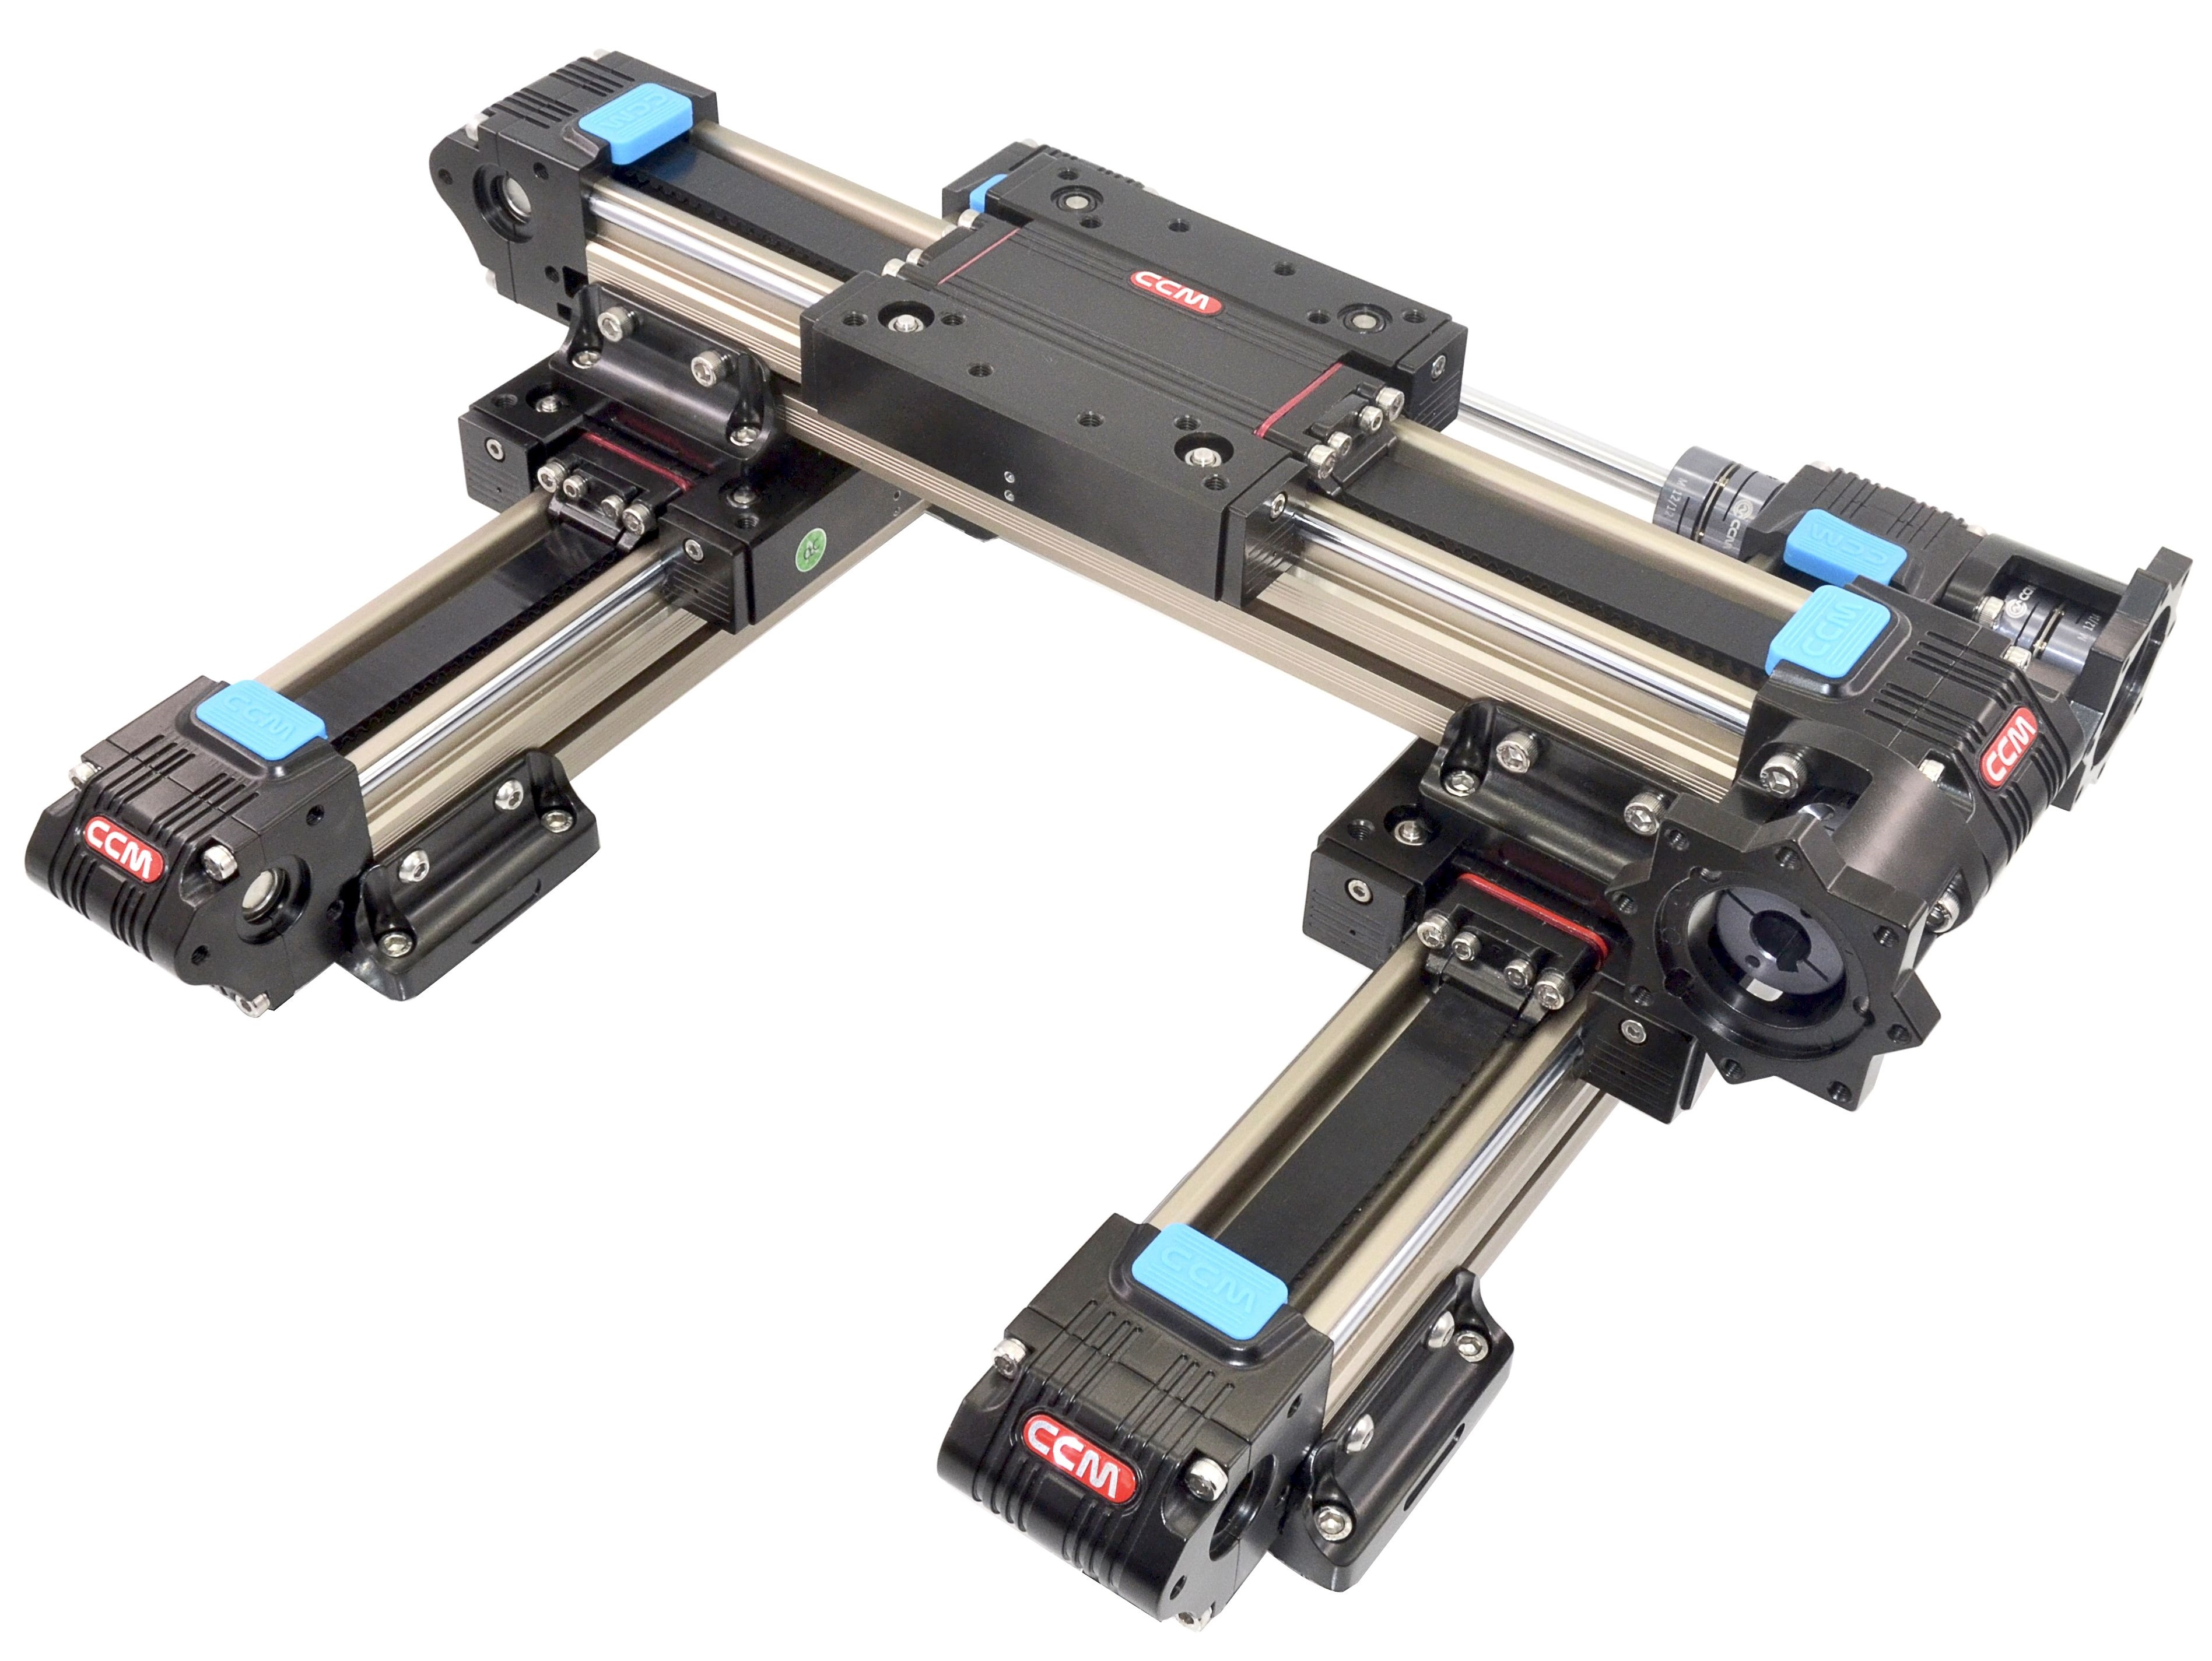
\includegraphics[scale = 0.03]{figuras/mcorreia}
        \end{figure}
\end{columns}

\end{frame}
    
% SLIDE DE MESA DE POSICIONAMENTO
\begin{frame}
\frametitle{Mesa de posicionamento}

Outro componente importante é o acionador, que pode ser um motor de passo. 

Os motores de passo são máquinas utilizadas em aplicações de um alto grau de precisão no movimento em passos fixos, referentes a uma fração de ângulo. 

\begin{figure}
\centering
\includegraphics[scale = 0.07]{figuras/motordepassoex}
\end{figure}
\end{frame}


\section{Metodologia}

\subsection{Sistema mecânico}

\subsubsection{Estrutura}

% SLIDE DE ESTRUTURA
\begin{frame}
\frametitle{Estrutura}

\begin{figure}
\centering
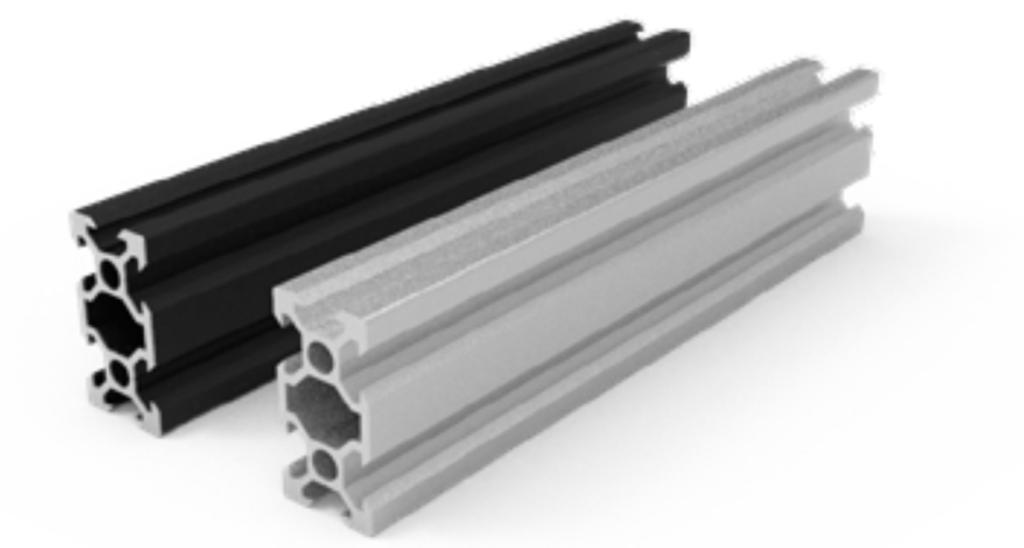
\includegraphics[scale = 0.15]{figs/p20x40p}
\end{figure}

\begin{figure}
\centering
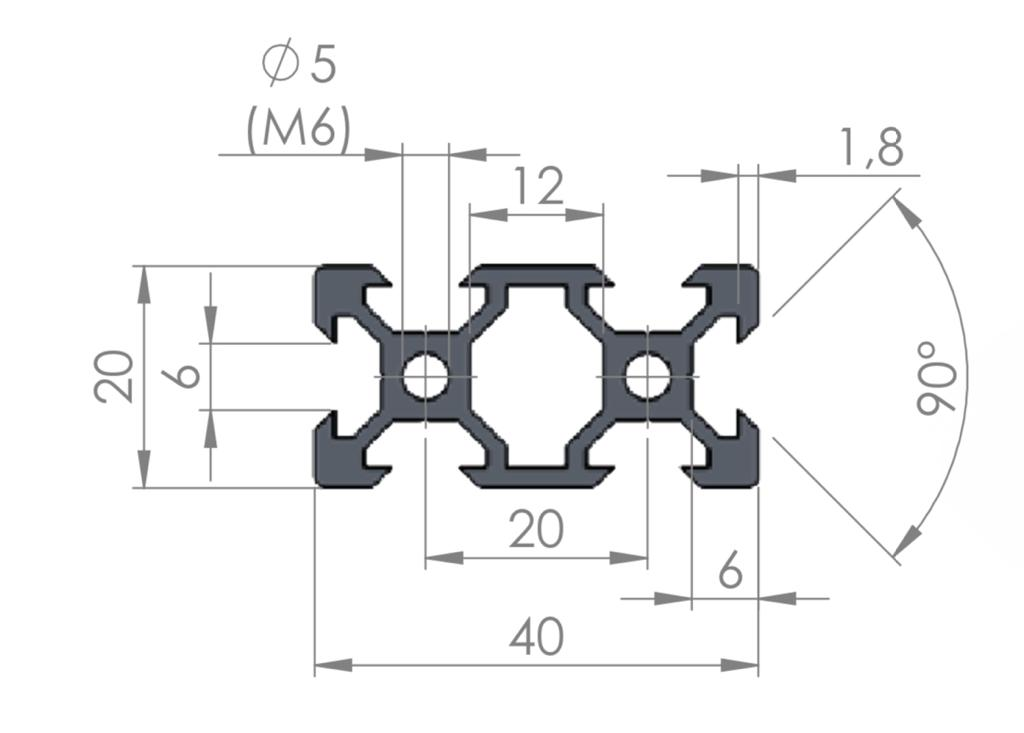
\includegraphics[scale = 0.15]{figs/p20x40d.jpeg}
\end{figure}
    
\end{frame}
    
% SLIDE DE ESTRUTURA
\begin{frame}
\frametitle{Estrutura}

\begin{figure}
\centering
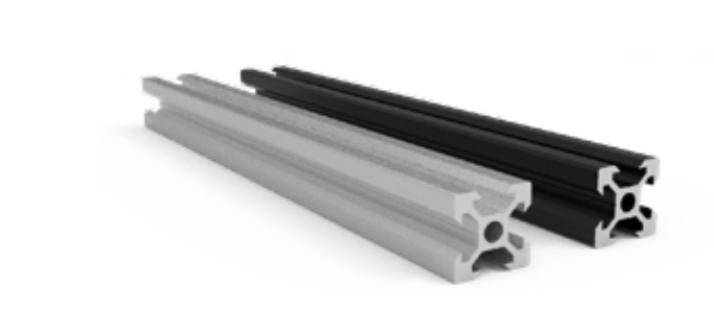
\includegraphics[scale = 0.25]{figs/p20x20p}
\end{figure}

\begin{figure}
\centering
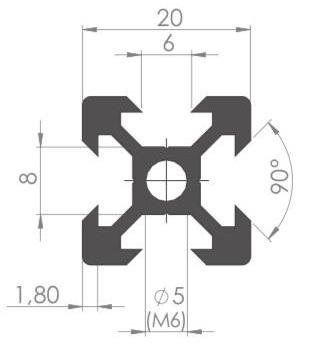
\includegraphics[scale = 0.45]{figs/p20x20d}
\end{figure}
    
\end{frame}

% SLIDE DE ESTRUTURA
\begin{frame}
\frametitle{Estrutura}

\begin{figure}
\centering
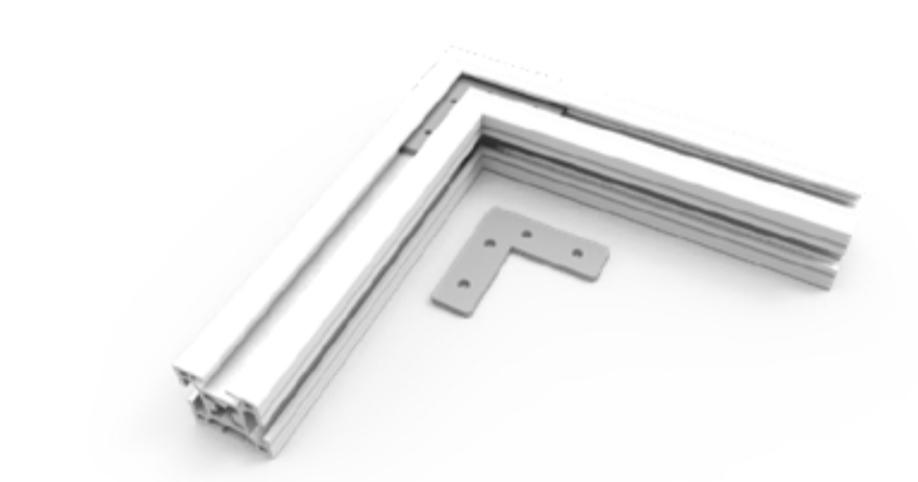
\includegraphics[scale = 0.15]{figs/pconexao90p}
\end{figure}

\begin{figure}
\centering
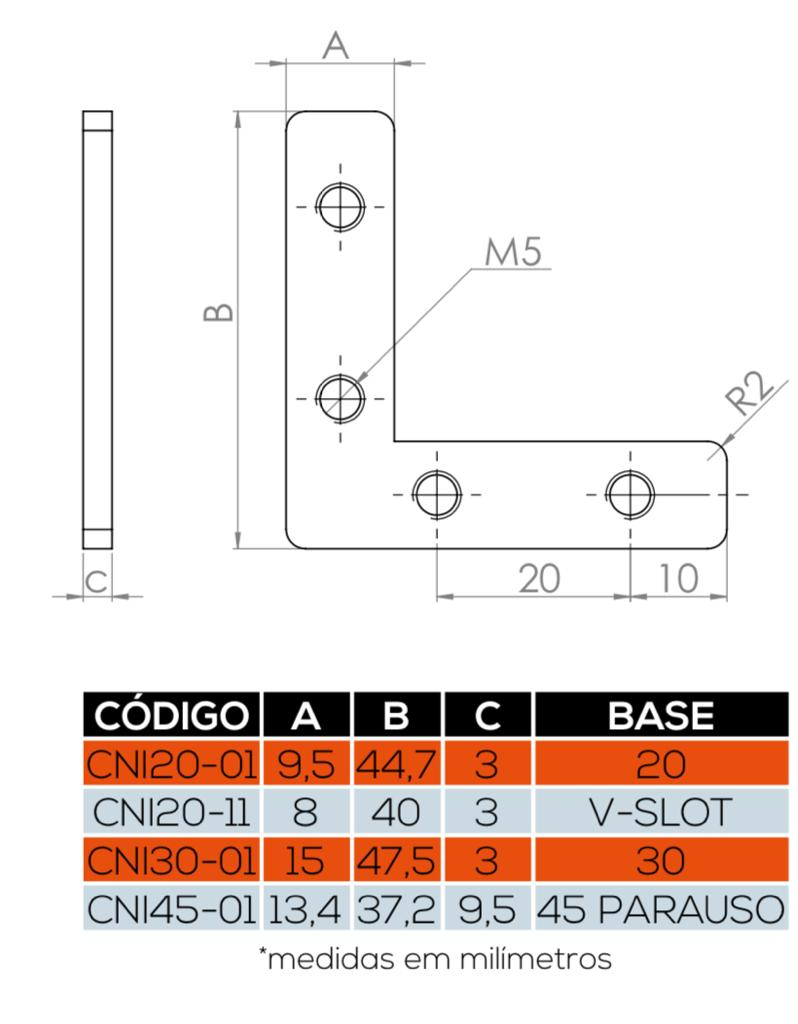
\includegraphics[scale = 0.15]{figs/pconexao90d}
\end{figure}
    
\end{frame}

% SLIDE DE ESTRUTURA
\begin{frame}
\frametitle{Estrutura}

\begin{figure}
\centering
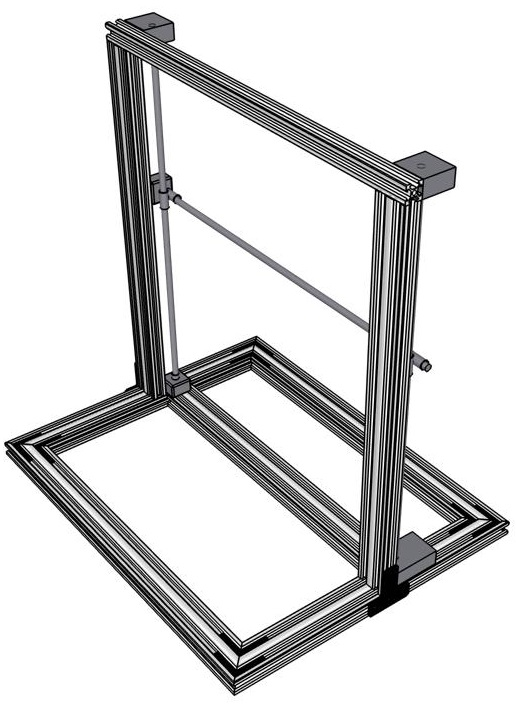
\includegraphics[scale = 0.4]{figs/estruturamesa}
\end{figure}  

\end{frame}
    
% SLIDE DE ESTRUTURA
\begin{frame}
\frametitle{Estrutura}

\begin{figure}
\centering
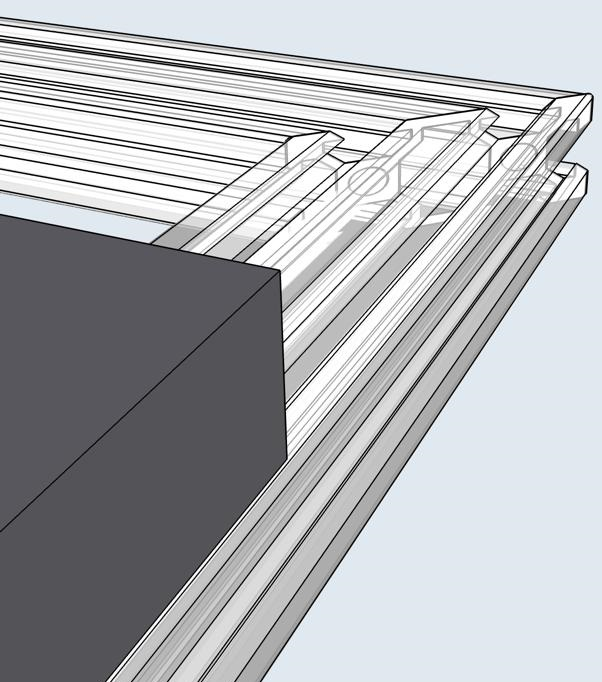
\includegraphics[scale = 0.4]{figs/detalhe45}
\end{figure}  
    
\end{frame}

% SLIDE DE ESTRUTURA
\begin{frame}
\frametitle{Estrutura}

\begin{figure}
\centering
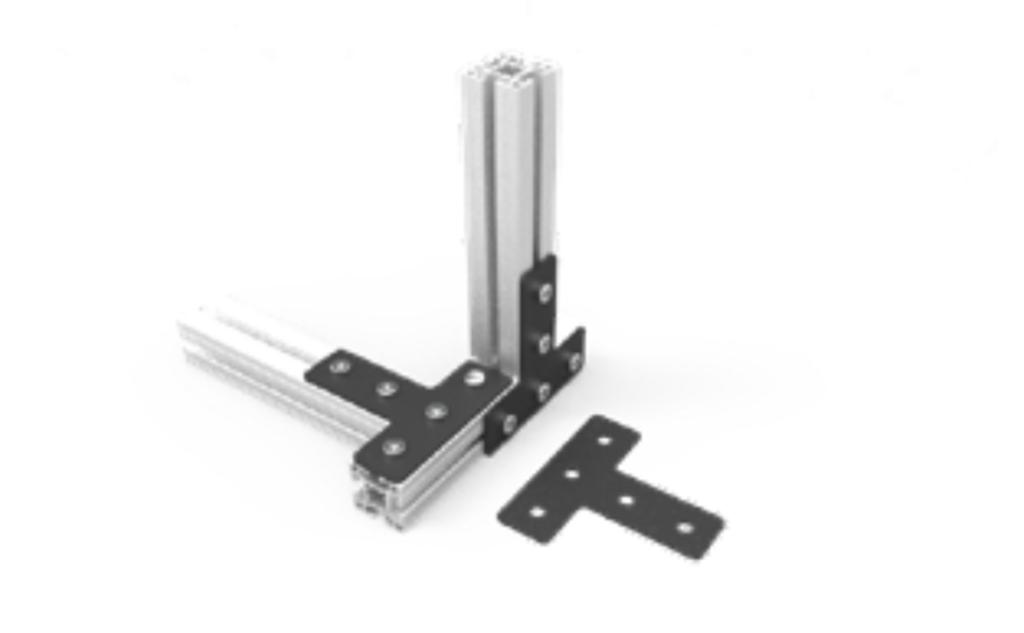
\includegraphics[scale = 0.10]{figs/placatp}
\end{figure}

\begin{figure}
\centering
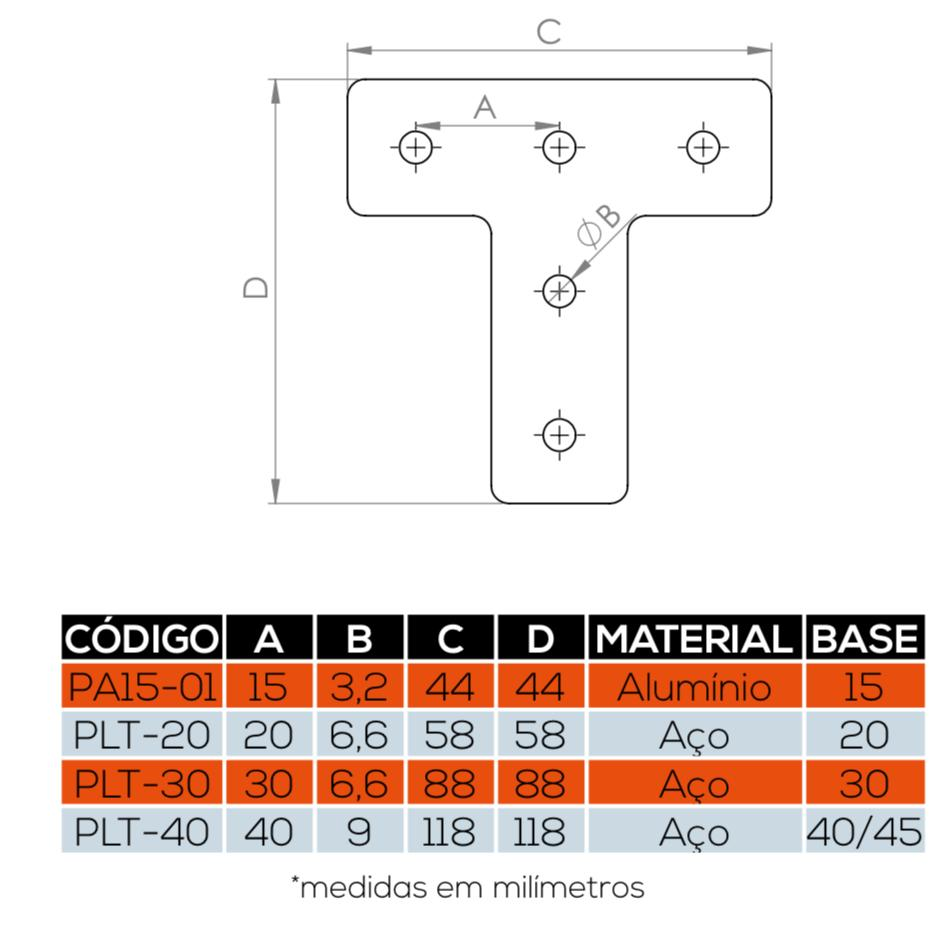
\includegraphics[scale = 0.10]{figs/placatd}
\end{figure}
    
\end{frame}

\subsubsection{Sistema de transmissão}

% SLIDE DE SISTEMA DE TRANSMISSÃO
\begin{frame}
\frametitle{Sistema de transmissão}

O sistemas de transmissão de potência  será dado por meio de fuso trapezoidal. 
O fuso terá as seguintes características:

\begin{itemize}
    \item Rosca TR8x8mm
    \item Passo 2mm com 4 entradas
    \item Avanço de 8mm por volta,  permitindo um deslocamento rápido.  
\end{itemize}

\begin{figure}
\centering
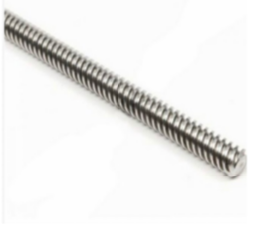
\includegraphics[scale = 0.8]{figs/fusotrapezoidal}
\end{figure}
    
\end{frame}

\subsubsection{Acionador}

% SLIDE DE ACIONADOR
\begin{frame}
\frametitle{Acionador}

O acionamento do sistema de transmissão será feito através de motores de passo, serão utilizados dois motores para o deslocamento vertical e um motor para o deslocamento horizontal.  

\begin{figure}
\centering
\includegraphics[scale = 0.1]{figs/motordepassoex}
\end{figure}
    
\end{frame}

    
\subsection{Sistema eletrônico}

\subsubsection{Diagrama de blocos do sistema eletrônico}

% SLIDE DE FLUXOGRAMA DO SISTEMA ELETRÔNICO
\begin{frame}
\frametitle{Diagrama de blocos do sistema eletrônico}

\begin{figure}
\centering
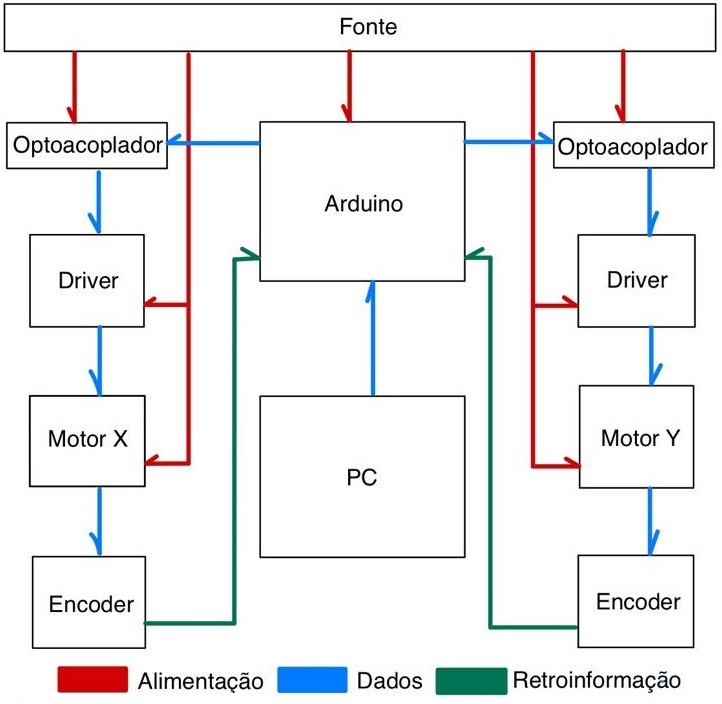
\includegraphics[scale = 0.30]{figuras/fluxogramaeletronico}
\end{figure}
    
\end{frame}

\subsubsection{Placa de prototipagem eletrônica Arduino}

% SLIDE DE PLACA DE PROTOTIPAGEM ELETRÔNICA ARDUINO
\begin{frame}
\frametitle{Placa de prototipagem eletrônica Arduino}

Funções:

O sistemas de transmissão de potência será dado por meio de fuso trapezoidal. 
O fuso terá as seguintes características:

\begin{itemize}
    \item Recepção e tratamento dos dados provenientes da interface computacional;
    \item O controle dos motores está fundamentado na programação do microcontrolador de acordo com as necessidades definidas inicialmente para operação da mesa cartesiana.
\end{itemize}

\end{frame}
    
% SLIDE DE PLACA DE PROTOTIPAGEM ELETRÔNICA ARDUINO
\begin{frame}
\frametitle{Placa de prototipagem eletrônica Arduino}

\begin{figure}
\centering
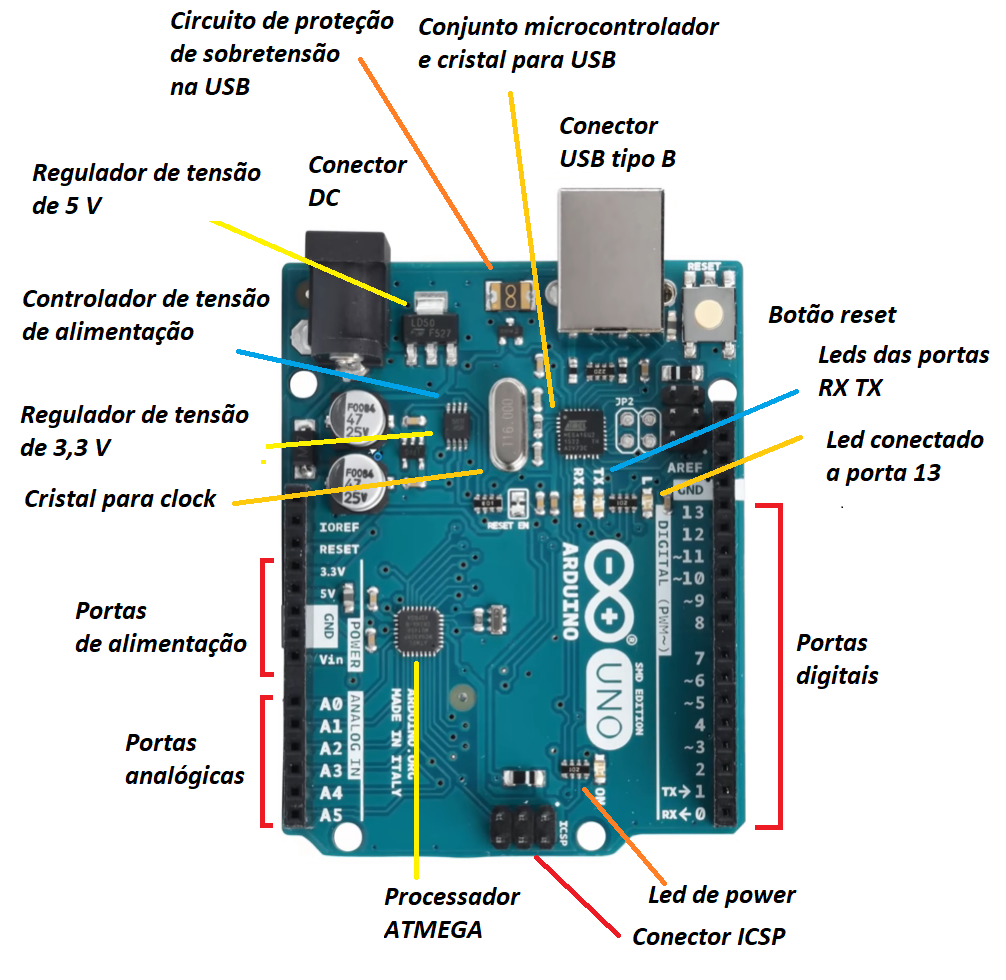
\includegraphics[scale = 0.3]{figs/placaarduino}
\end{figure}

\end{frame}

\subsubsection{Drivers de potência}

% SLIDE DE DRIVERS DE POTÊNCIA
\begin{frame}
\frametitle{Drivers de potência}

Os drivers têm a função de, a partir dos sinais originados pelo Arduino, atender a demanda dos motores de passo utilizados.

\begin{figure}
\centering
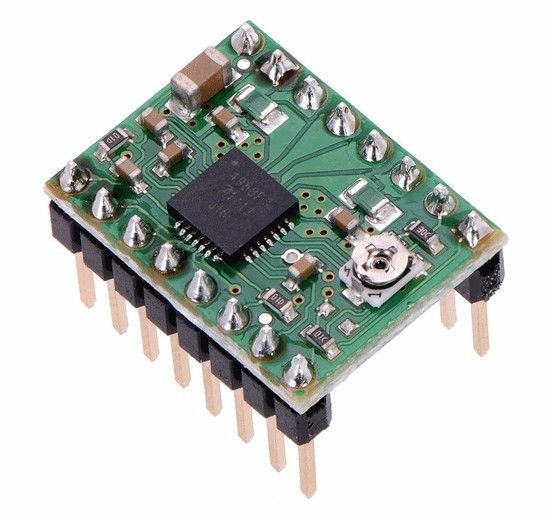
\includegraphics[scale = 0.2]{figs/driver}
\end{figure}

\end{frame}

\subsubsection{Atuadores}

% SLIDE DE ATUADORES
\begin{frame}
\frametitle{Atuadores}

O motor de passo foi escolhido para esse projeto devido a sua capacidade de realizar passos, que são rotações discretas incrementais e precisas. 

\begin{figure}
\centering
\includegraphics[scale = 0.1]{figuras/motordepassoex}
\end{figure}

\end{frame}

% SLIDE DE ATUADORES
\begin{frame}
\frametitle{Atuadores}

Os passos são definidos por um número fixo de pólos magnéticos de dente de engrenagens do motor determinando assim, a precisão de ângulo de rotação do motor de passo.

\begin{figure}
\centering
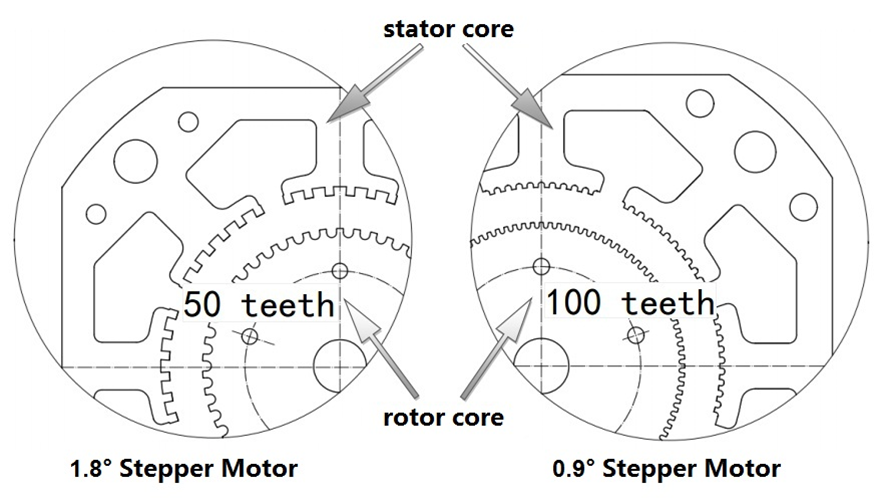
\includegraphics[scale = 0.2]{figuras/didaticopasso}
\end{figure}

\end{frame}

% SLIDE DE ATUADORES
\begin{frame}
\frametitle{Atuadores}
\centering

\begin{figure}
\centering
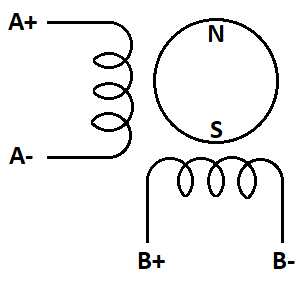
\includegraphics[scale = 0.4]{figuras/meumotorbipolar}
\end{figure}
    
\begin{tabular}{cccccc}
    \hline
    \textbf{Passo} & \textbf{A+} & \textbf{B+} & \textbf{A-} & \textbf{B-} & \textbf{Decimal}\\
    \hline
    1 & 0 & 0 & 0 & 1 & 1\\
    2 & 0 & 0 & 1 & 0 & 2\\
    3 & 0 & 1 & 0 & 0 & 4\\
    4 & 1 & 0 & 0 & 0 & 8\\        
    \hline       
\end{tabular}
\end{frame}

\subsubsection{Fonte de alimentação}

% SLIDE DE FONTE DE ALIMENTAÇÃO
\begin{frame}
\frametitle{Fonte de alimentação}

Para a escolha correta da fonte de alimentação é necessário definir a demanda de energia elétrica que os dispositivos que são alimentados pela fonte necessitam.

Conforme a determinação da tensão de saída e o cálculo de corrente necessária, é possível determinar que a fonte deve ter 12 V e 10,64 A.

\begin{figure}
\centering
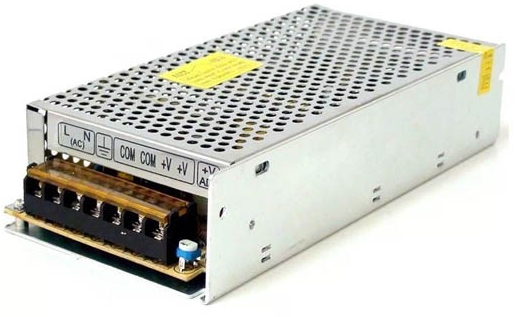
\includegraphics[scale = 0.5]{figs/fonte}
\end{figure}

\end{frame}

\subsubsection{Acopladores ópticos}

% SLIDE DE ACOPLADORES ÓPTICOS
\begin{frame}
\frametitle{Acopladores ópticos}

Os acopladores ópticos são dispositivos que operam por meio de um feixe de luz, 
para transmitir sinais de um circuito para outro.
O led emite um sinal infra vermelho, o foto transistor capta e satura,
conduzindo corrente do coletor para o emissor.

\begin{figure}
\centering
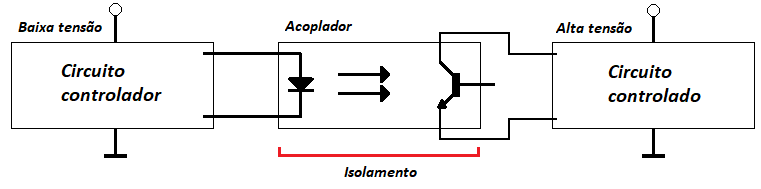
\includegraphics[scale = 0.4]{figuras/acoplador}
\end{figure}

\begin{figure}
\centering
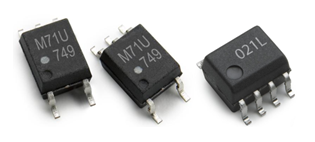
\includegraphics[scale = 0.2]{figuras/fotoacoplador}
\end{figure}

\end{frame}

\subsubsection{Encoders}

% SLIDE DE ENCODERS
\begin{frame}
\frametitle{Encoders}

Responsáveis pelo sistema de controle de posição transformando a medida de posição em sinal elétrico digital transmitida à placa controladora.

\begin{figure}
\centering
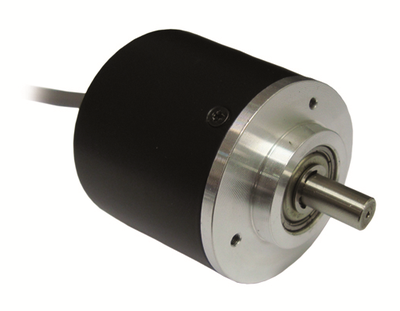
\includegraphics[scale = 0.5]{figuras/encoder}
\end{figure}

\end{frame}

\subsubsection{Chaves Fim de curso}

% SLIDE DE CHAVES FIM DE CURSO
\begin{frame}
\frametitle{Chaves fim de curso}

Limitação de campo de movimento de eixos, como os presentes na mesa cartesiana. Tem a capacidade de mudança de estado de conexão em circuitos, alternando o estado de aberto para fechado e vice-versa.

\begin{figure}
\centering
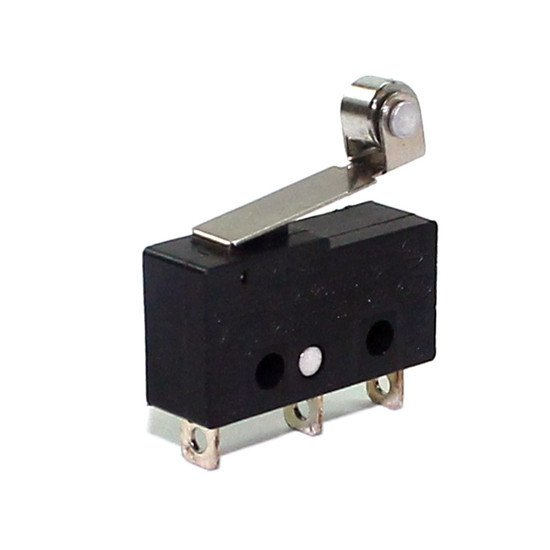
\includegraphics[scale = 0.3]{figs/chavefimdecurso}
\end{figure}

\end{frame}

\subsubsection{Diagrama de blocos do sistema eletrônico com imagens}

% SLIDE DE FLUXOGRAMA DO SISTEMA ELETRÔNICO COM IMAGENS
\begin{frame}
\frametitle{Diagrama de blocos do sistema eletrônico}

\begin{figure}
\centering
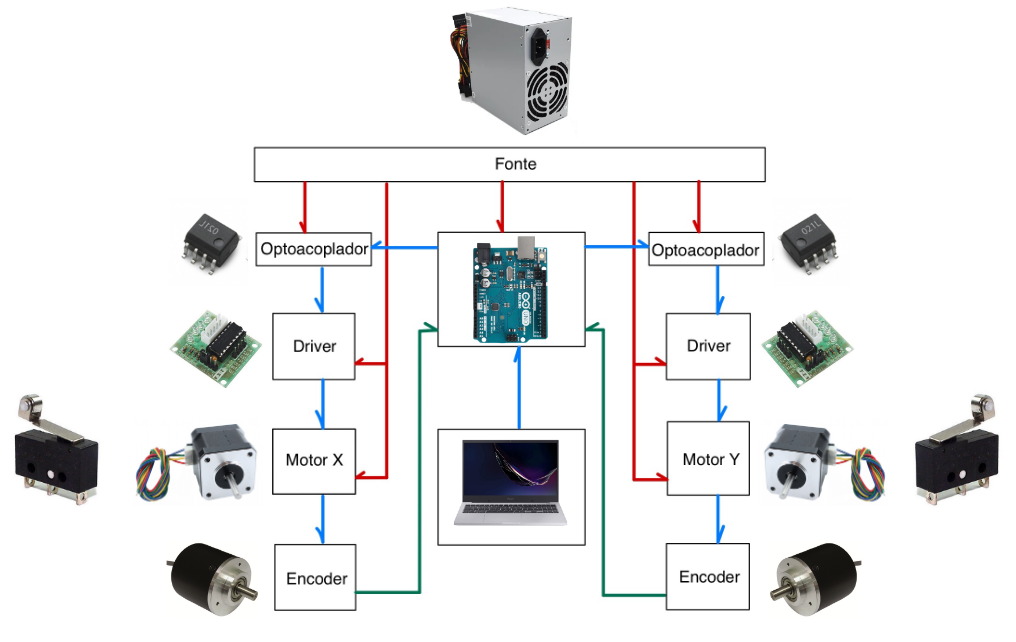
\includegraphics[scale = 0.30]{figuras/diagramblocoscomimagens}
\end{figure}

\end{frame}


\subsection{Sistema de software}

\subsubsection{Plataforma de prototipação Arduino IDE}

% SLIDE DE PLATAFORMA DE PROTOTIPAÇÃO ARDUINO IDE
\begin{frame}
\frametitle{Plataforma de prototipação Arduino IDE}

É um software que permite o desenvolvimento e envio de códigos compilados direto para o microcontrolador.

\begin{figure}
\centering
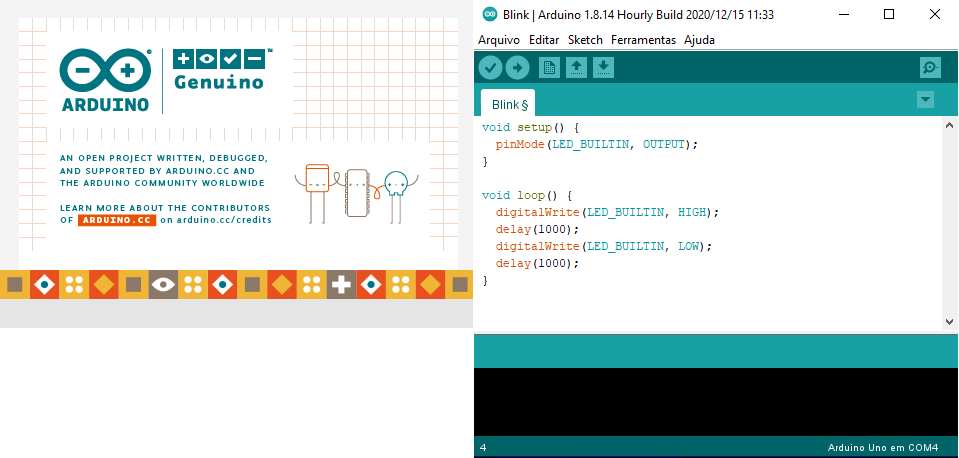
\includegraphics[scale = 0.3]{figuras/idearduino}
\end{figure}

\end{frame}

\subsubsection{Lógica de programação}

% SLIDE DE LÓGICA DE PROGRAMAÇÃO
\begin{frame}
\frametitle{Lógica de programação}

\begin{figure}
\centering
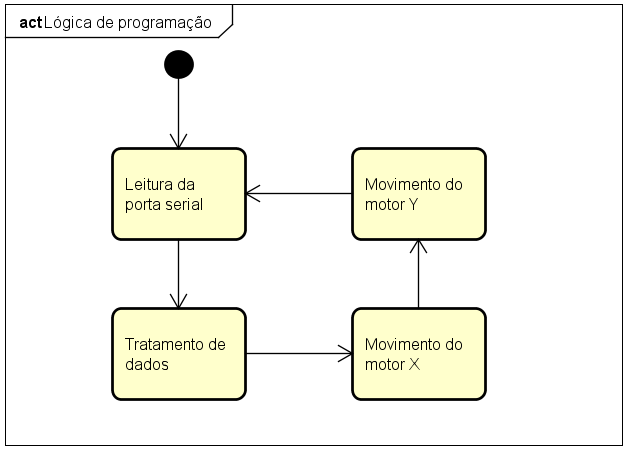
\includegraphics[scale = 0.45]{figuras/fluxoexecucao}
\end{figure}

\end{frame}

\subsubsection{Diagrama de classes}

% SLIDE DE DIAGRAMA DE CLASSES
\begin{frame}
\frametitle{Diagrama de classes}

\begin{figure}
\centering
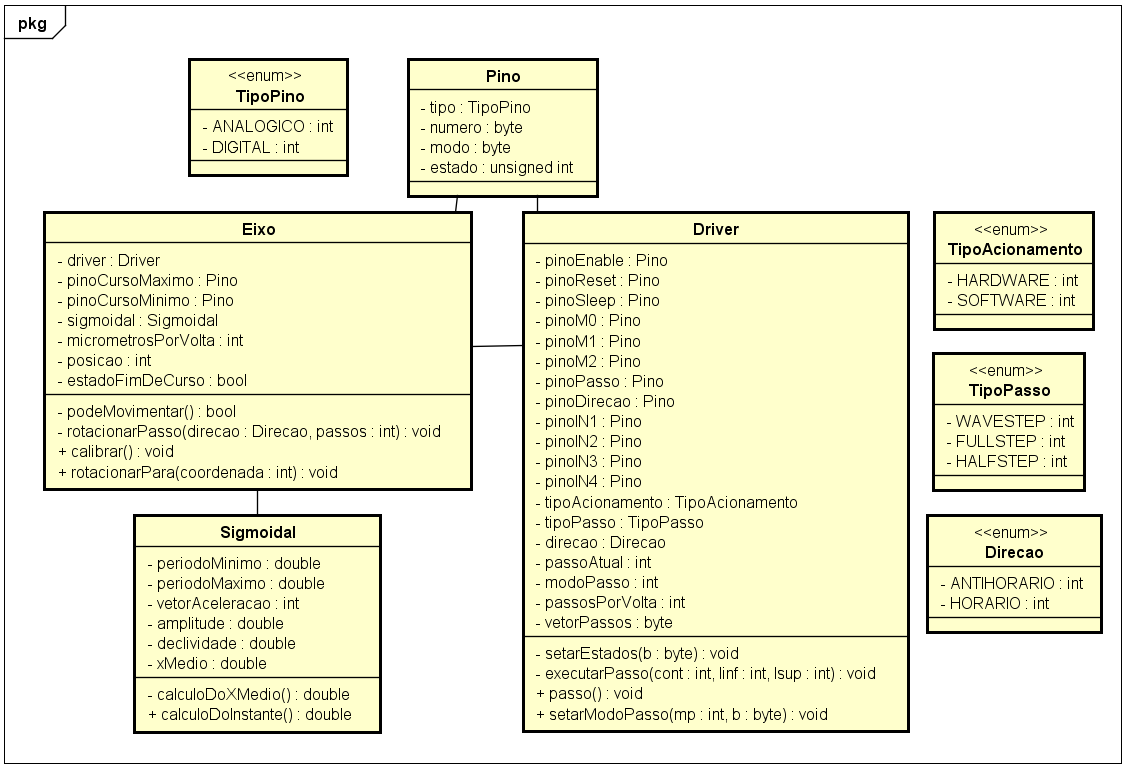
\includegraphics[scale = 0.35]{figs/diagramaclasses}
\end{figure}

\end{frame}

\subsubsection{Organização geral do software}

% SLIDE DE ORGANIZAÇÃO GERAL DO SOFTWARE
\begin{frame}
\frametitle{Organização geral do software}

\begin{figure}
\centering
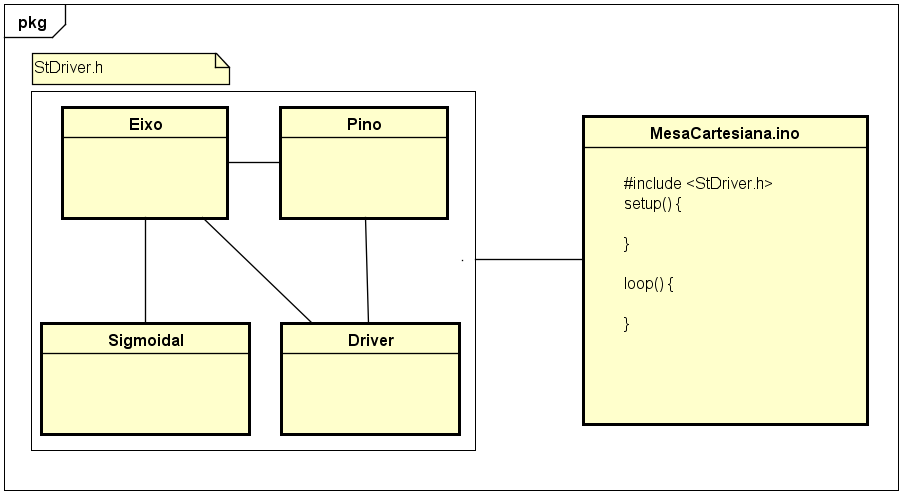
\includegraphics[scale = 0.4]{figs/orgsoftware}
\end{figure}

\end{frame}


\subsection{Integração dos sistemas}

\subsubsection{Integração dos sistemas}

% SLIDE DE INTEGRAÇÃO DOS SISTEMAS
\begin{frame}
\frametitle{Integração dos sistemas}

\begin{figure}
\centering
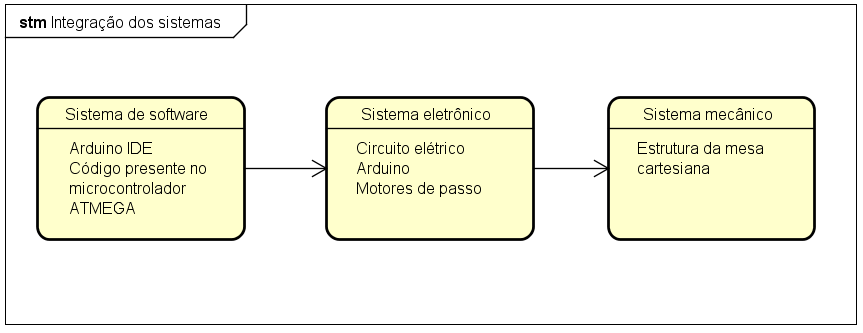
\includegraphics[scale = 0.4]{figuras/integracao}
\end{figure}

\end{frame}


\section{Resultados e discussão}
    
\section{Considerações finais}

\end{document}